
\chapter[Tia X]{Tia X}
\section{Lý thuyết}
\subsection{Bản chất}

Tia X (còn gọi là tia R\"ontgen) là sóng điện từ có bước sóng rất ngắn (từ $10^{-8}\ \text{m}$ đến $10^{-11}\ \text{m}$).

\subsection {Cách tạo ra}
Tia X được tạo thành từ ống phóng tia X:
\begin{itemize}
	\item Các electron từ cathode được tăng tốc trong điện trường mạnh sẽ có động năng lớn.
	\item Khi electron đập vào đối cathode, chúng xuyên qua lớp vỏ nguyên tử, tương tác với hạt nhân và các electron ở bên trong làm phát ra sóng điện từ có bước sóng cực ngắn, gọi là tia X.
	
	\begin{center}
		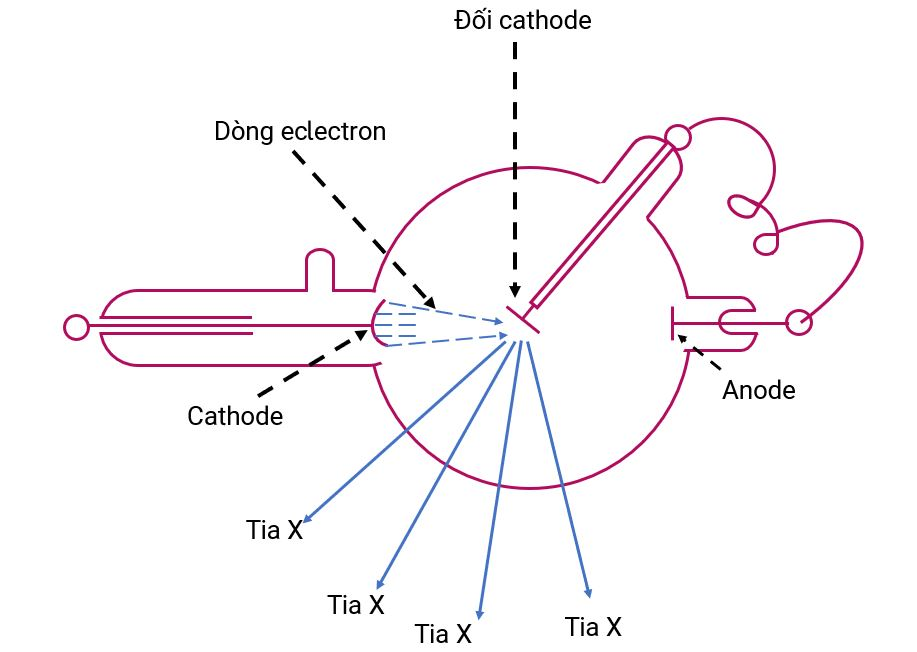
\includegraphics[scale=0.5]{../figs/VN12-PH-36-L-021-5-1.JPG}
	\end{center}
\end{itemize}
Ngoài ra, tia X còn được tạo thành do quá trình va chạm trong các khối khí có nhiệt độ rất cao (Mặt trời, các sao,...)
\subsection{Tính chất}

Tia X có các tính chất:

\begin{itemize}
	\item Tính chất nổi bật nhất là khả năng đâm xuyên qua giấy, vải, gỗ thậm chí cả kim loại. Tia X có bước sóng càng ngắn thì càng xuyên được sâu hay càng cứng.
	\item Tác dụng mạnh lên kính ảnh.
	\item Làm ion hóa không khí. 
	\item Làm phát quang một số chất.
	\item Tác dụng sinh lý: làm hủy họa tế bào, diệt vi khuẩn,..
	
\end{itemize}

\subsection{Ứng dụng}

\begin{itemize}
	\item Y học: sử dụng để chiếu điện, chụp điện, chữa ung thư nông.
	\item Công nghiệp: kiểm tra chất lượng bên trong sản phẩm.
	\item Giao thông: kiểm tra hành lý của hành khách.
	\item Phòng thí nghiệm: nghiên cứu cấu trúc vật rắn.
\end{itemize}
\section{Bài tập tự luyện}
\begin{enumerate}[label=\bfseries Câu \arabic*:]
	
	%=======================================
	\item \mkstar{1} [9]
	\cauhoi
	{Tia \textbf{X} không có tính chất nào sau đây?
		\begin{mcq}(2)
			\item Tác dụng lên phim ảnh. 
			\item Đâm xuyên qua tất cả các kim loại. 
			\item Gây ra quang điện cho hầu hết kim loại. 
			\item Làm phát quang các chất. 
		\end{mcq}
	}
	
	\loigiai
	{		\textbf{Đáp án: B.}
		
		Tia X không thể xuyên qua tấm chì vài centimét.
	}
	
	%=======================================
	\item \mkstar{1} [4]
	\cauhoi
	{Phát biểu nào \textbf{đúng} về tia X?
		\begin{mcq}(1)
			\item Tia X có khả năng đâm xuyên kém hơn tia hồng ngoại.. 
			\item Tia X có tần số nhỏ hơn tần số của tia hồng ngoại. 
			\item Tia X có bước sóng lớn hơn bước sóng ánh sáng nhìn thấy. 
			\item Tia X có tác dụng sinh lí, nó hủy diệt tế bào. 
		\end{mcq}
	}
	
	\loigiai
	{		\textbf{Đáp án: D.}
		
		Tia X có tác dụng sinh lí, nó hủy diệt tế bào. 
	}
	
	%=======================================
	\item \mkstar{1} [10]
	\cauhoi
	{Tia Rơnghen có 
		\begin{mcq}(1)
			\item cùng bản chất với sóng âm. 
			\item bước sóng lớn hơn bước sóng của tia hồng ngoại. 
			\item cùng bản chất với sóng vô tuyến. 
			\item điện tích âm. 
		\end{mcq}
	}
	
	\loigiai
	{		\textbf{Đáp án: C.}
		
		Tia Rơnghen có cùng bản chất với sóng vô tuyến.
	}
	
	%=======================================

	%=======================================
	\item \mkstar{1} [7]
	\cauhoi
	{Khi nói về tia X, phát biểu nào sau đây là \textbf{đúng}?
		\begin{mcq}(1)
			\item Tia X có tần số nhỏ hơn tia hồng ngoại. 
			\item Tia X có cùng bản chất với tia Catốt.
			\item Tia X có khả năng đâm xuyên mạnh. 
			\item Tia X có bước sóng lớn hơn bước sóng của ánh sáng nhìn thấy.
		\end{mcq}
	}
	
	\loigiai
	{		\textbf{Đáp án: C.}
		
		Tia X có khả năng đâm xuyên mạnh.
	}
	
	%=======================================
	\item \mkstar{1} [3]
	\cauhoi
	{Phát biểu nào sau đây là \textbf{sai}?
		\begin{mcq}(1)
			\item Tia X có bước sóng nhỏ hơn bước sóng của ánh sáng tím. 
			\item Tia X có tác dụng sinh lý. 
			\item Tia X làm ion hóa không khí. 
			\item Tia X có bước sóng lớn hơn bước sóng của tia hồng ngoại. 
		\end{mcq}
	}
	
	\loigiai
	{		\textbf{Đáp án: D.}
		
		Tia X có bước sóng lớn hơn bước sóng của tia hồng ngoại là sai. 
	}
	
	%=======================================
	\item \mkstar{1} [2]
	\cauhoi
	{Tia X được tạo ra bằng cách nào sau đây?
		\begin{mcq}(1)
			\item Cho electron có động năng lớn đập vào một kim loại có nguyên tử lượng lớn. 
			\item Chiếu tia tử ngoại vào kim loại có nguyên tử lượng lớn. 
			\item Chiếu một chùm ánh sáng nhìn thấy vào một kim loại có nguyên tử lượng lớn. 
			\item Chiếu tia hồng ngoại vào một kim loại có nguyên tử lượng lớn. 
		\end{mcq}
	}
	
	\loigiai
	{		\textbf{Đáp án: A.}
		
		Tia X được tạo ra bằng cách cho electron có động năng lớn đập vào một kim loại có nguyên tử lượng lớn. 
	}
		\item \mkstar{1} 
	\cauhoi
	{Tìm kết luận sai. Để phát hiện ra tia X, người ta dùng
		
		\begin{mcq}(2)
			\item màn huỳnh quang. 	
			\item   máy đo dùng hiện tượng ion hóa.
			
			\item tế bào quang điện. 	
			\item mạch dao động $LC$.
			 
		\end{mcq}
	}
	
	\loigiai
	{		\textbf{Đáp án: D.}
		
		 Bước sóng tia X rất nhỏ so với sóng vô tuyến, để phát hiện tia X không dùng mạch dao động $LC$. 
	}
	\item \mkstar{1} 
	\cauhoi
	{Tia X không có ứng dụng nào sau đây?
		
		\begin{mcq}(1)
			\item Chữa bệnh ung thư.	
			\item Tìm bọt khí bên trong các vật bằng kim loại.
			\item Chiếu điện, chụp điện.
			\item  Sấy khô, sưởi ấm.
		\end{mcq}
	}
	
	\loigiai
	{		\textbf{Đáp án: D.}
		
		Tia X không có tác dụng nhiệt nổi bật và có khả năng huỷ hoại tế bào nên không có ứng dụng sấy khô, sưởi ấm.
	}
\end{enumerate}


